\chapter{Modelling And Meaning Representation}
\label{sec:concepts}


In this chapter, we address the concepts and the theoretical framework for modelling meaning with uncertainty and grounding natural language in multi-modal representations.

\section{Terminology of modelling}
\label{sec:concepts:model}
Whenever we need to make a systematic prediction based on observations and evidence, we use a set of assumptions. 
A \emph{model} is the encoding of these assumptions in the form of a function. 
This function takes given evidence as input and produces the prediction as an output. Formally, modelling $y$ based on $x$ with the function $f$ would be as follows:

\begin{equation}
y = f_{\Theta}(x)
\end{equation}
\noindent where $f_{\Theta}$ is called the \emph{model function}, which is parametrised with $\Theta$. 

The parameters are part of the assumption about the model function. 
For example, by assuming the rules of physics, the position of a falling object at a specific time in the future can be modelled given the current evident position of the object. 
However, the formula of the location still requires the important parameters of velocity and acceleration of the object in the model. 
More often, determined prediction of an outcome is not enough. We need to associate each prediction with an uncertainty measure. 
Such a model is a \emph{probabilistic model}. 
Instead of modelling the predictable outcome, a measure of uncertainty for any possible outcome is modelled; the density of possible outcomes is conditioned with the observable evidence.
\begin{equation}\label{eq:probabilistic_model}
\mathrm{Pr}( Y=y | X=x ) = f_{\Theta}(y, x)
\end{equation}
\noindent where $f_{\Theta}$ is the model function, which assigns a degree of uncertainty for predicting $y$ grounded on an observable $x$. To simplify the probability annotations, we do not write the complete propositions ($Y=y$); instead, we use shorthand \textemdash  $\mathrm{Pr}( y | x )$.
Commonly, the probability distributions used in this work are categorical, in which $Y$ is a bounded discrete vector of the items. Therefore, the common implementation of function $f_{\Theta}$ is conducted using a module with a vectorised output the same size as $Y$:
\begin{equation}\label{eq:probabilistic_model_module}
f_{\Theta}(y, x) = \mathtt{modules}(x)[y]
\end{equation}
\noindent where $y$ is a category in distribution, the output of $\mathtt{modules}(.)$ is a vector with the size of all possible categories and the square bracket annotation $[y]$ indicates a lookup operation to select the value for $y$-key.

Representing assumptions about the future in a function requires a \emph{framework of modelling} to acquire the model function. 
A constructive \emph{proof}, a search algorithm over a class of functions or its parameters, is the path to building the model function from these assumptions.
When a set of data points drives the search algorithm, the process of fitting a function according to these data points is called \emph{learning} or \emph{training} the model.


\section{Modelling in deep neural networks}
\label{sec:concepts:dl}
In this work, we study the framework of artificial neural networks to encode and build the model function. 
\emph{Deep learning} (DL) and \emph{artificial neural networks} (ANN)
refer to a modelling framework in which a composition of differentiable functions form the model function.
The learning occurs through parameters of the function with the \emph{backpropagation algorithm}.
The backpropagation algorithm is a data-driven optimisation algorithm that uses a measure of error loss over the training data to gradually update the model parameters toward lower error. 
The differentiability of the loss enables this method to apply the chain rule of derivatives to aim the parameter updates toward reducing errors for the training data. 
In a nutshell, the critical assumptions needed to build a deep learning model are the assumed model function (the composition of modules or the neural network architecture), the assumption that the training dataset has relevant knowledge for the task and the assumption about the error function (the loss function).

There are several learning paradigms, such as supervised and unsupervised learning.
These distinctions mainly concern the difference in annotation on the training data, the error function and how they are related to the predictable variable of the model.
The most common paradigm is supervised learning, in which the training dataset is a set of annotated inputs and the predicted output of the model $D = \{(y_i, x_i)\}$.
Unsupervised learning, on the other hand, uses an unlabelled training dataset $D = \{x_i\}$.
The error function in these cases provides additional assumptions about how data points are internally connected. Any internal data structures that indirectly relate to the predictable outcome of the model could be the basis for an error function in unsupervised learning, such as unsupervised clustering of data points for a classification task without supervised data.

The most common loss function for deep learning models is the surprisal of the training data. The surprisal of a random variable ($X=x$) is defined as: 
$\bm{I}_X(x) = -\mathrm{log}(\mathrm{Pr}(X=x))$. 
With a given dataset, such as $D = \{(y_i, x_i)\}$ and a model function $f$, an ideal search algorithm for finds the best fitting parameters that minimise the loss:
\begin{align}
J_\Theta(f,D) &= \sum_{(y_i, x_i) \in D}{-\mathrm{log}(f_{\Theta}(y_i, x_i))} \\
\Theta &= \underset{\Theta}{\mathrm{argmin}} J_\Theta(f,D)
\end{align}
\noindent while the search algorithm looks for the best fitting parameters $\Theta$, there is usually more than one answer or there is no converging path to an acceptable error level with backpropagation. In the most straightforward form \textemdash  backpropagation in a \emph{gradient descent algorithm} \textemdash  the gradient of the error function with a pre-defined learning rate updates all parameters iteratively until the error converges to an acceptable threshold. 
To overcome technical difficulties in processing large datasets and parameter space, other variations of this algorithm may process data in batches, using \emph{stochastic gradient descent} and the momentum of past updates. 
For simplicity, each step of mini-batch training can be formulated as an updating operation for $\Theta$ parameters as follows: 
\begin{equation*}
\Theta = \Theta - \eta \cdot \nabla_\Theta J_\Theta(f; D_{batch})
\end{equation*}
\noindent
where $\eta$ is a hyper-parameter for the learning rate and $\nabla_\Theta$, is a notation for a stochastic deferential operation over every parameter in $\Theta$.

The concept of indirect learning from a function different from the goal prediction of the model is also related to the concept of \emph{multi-task learning} and \emph{transfer learning} in neural networks \citep[Chapter~15]{Goodfellow-et-al-2016}. 
In summary, the parameters of a model function learned from a different dataset or a different goal or a different task encode relevant assumptions needed to make our intended prediction model.
Therefore, the pre-trained modules can be reused or composed into the model function in the neural network. 
The final training steps with much less training data is then known as fine-tuning or in some context referred to as domain adaptation phase.


\section{Grounding in representations}
\label{sec:concepts:grounding}
So far, we have identified that modelling is a way to represent assumptions about the world in the form of the parameters of a predicting function and that DL models encode assumptions inferred from data as a representation space.
The goal of understanding and comprehension is to connect two types of representations \textemdash sensory representations and abstract concepts.
A model that provides the link between two representations is a model of grounded meaning. 
A probabilistic model of representations can potentially formulate such links. 
However, the question remains about the generalisability of the learning (see section~\ref{sec:concepts:compositionality}).

By definition, the model represents the uncertainty of connecting observables to their representation; therefore, it can be used as a model of \emph{grounded representations}. 
Within the paradigms of DL, instead of having a given strict symbolic representation for concepts and their internal associations, these representations must be learned. 
The architectural design of the neural networks and the training datasets impose restrictions on how these representations are interconnected. 
In the machine learning community, this has become a field of study called \emph{representation learning} \citep{bengio2013representation}. 

When modelling conversational agents, linguistic expressions are grounded in internal representations of the agent. There are at least two probabilistic models of meaning for (1) generating and (2) understanding utterances:
\begin{align}
\mathrm{Speaker~model}:& \mathrm{Pr}(u | r) = f_{\Theta_s}(u, r) \label{ch3:eq:utt}\\
\mathrm{Listener~model}:& \mathrm{Pr}(r | u) = f_{\Theta_l}(u, r)
\end{align}
\noindent $\mathrm{Pr}(u | r)$ is the measure of uncertainty in choosing the utterance  $u$, referring to the given representation  $r$. 
$\mathrm{Pr}(r | u)$ is the measure of uncertainty in interpreting the given utterance $u$ as if it meant representation $r$ for the listener. 
In other words, the grounded meaning of each natural language utterance is what it denotes in the representation space according to the model.
Without any probabilistic sampling in composition of modules in neural networks, there is unambiguous mapping of sensory representations onto grounded representation space. 
However, the link between grounded representations and natural language utterances is uncertain, with a linking degree of uncertainty on all possible outcomes. 
The learning process establishes the degree of certainty of the link between utterances and representation space and builds the fitting map between the agent’s primitive sensory and motor representations and grounded representation space. 

Later, in section~\ref{sec:concepts:glm}, we provide additional discussion about the link between meaning and representations in the speaker model. 
In a speaker model, to express what is in an image, the sensory data for the situation is first mapped onto the representation space ($\raisebox{-0.3\height}{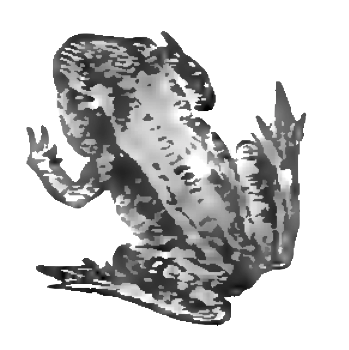
\includegraphics[width=0.5cm]{gfx/frog.png}} \Rightarrow v$). Then, the speaker model assigns a measure of goodness to the utterance predictions:
\begin{equation*}
\mathrm{Pr}(\mathrm{``there~is~a~frog"} | v) = f_{\Theta_s}([\mathrm{``there"},\mathrm{``is"},\mathrm{``a"},\mathrm{``frog"}], v)
\end{equation*}
\noindent In other words, the model of grounded meaning is also a model for connecting utterances to sensory evidence. 
The internal representations are not directly connected to external references. 
They are interpretations of the sensory readings internal to the agent. 
The mapping function between visual sensory inputs and internal agent representations could be modelled with a pre-trained convolutional network enriched with other contextual information about the situation. %
The model establishes uncertain links between primitive sensory readings and utterances of natural language, for that reason it functions as a model of grounding. 
In section~\ref{sec:concepts:convnets}, we describe some properties of this representation space and how sensory features would be mapped onto this representation space.




\section{Modelling compositionality}
\label{sec:concepts:compositionality}
One of the challenges of a model of grounding is formulated as Harnad’s symbol grounding problem \citep{harnad1990symbol}. 
The argument is that the capacity of learning from limited data is problematic when it is expected to impose new links to potentially unlimited compositions in a symbolic representation system.
The challenge is to infer grounded meanings for new representations (e.g. \textsc{`zebra'}) from known bottom-up representations learned from images (e.g. \textsc{`horse'} and \textsc{`stripes'}) 
when a symbolic link between them (\textsc{`zebra'} and a composition of two others) is established in natural language (\textsc{`zebra'} = \textsc{`horse'} + \textsc{`stripes'}).
In other words, compositionality as an ability to construct new representations linked to both sensory and abstract linguistic representations creates a generalisation problem for bottom-up learning.
The underlying premise of Harnad’s formulation of the problem is that human language is symbolic;
therefore, when human behaviour shows the capability of learning from language input, the establishment of such links came from new symbolic rules imposed by new statements of the natural language.

Without this explicit premise about the nature of language, the recent literature of language modelling stretches the notion of compositionality. 
In one account, any function in a semantic vector space is a model of compositionality \citep{mitchell2010composition}. 
In another direction, the semantic parse trees of linguistic expressions are used for composing neural network modules \citep{andreas2016neural}.

The notion of compositionality in natural language that we use in this thesis is simply the extent of generalisation in bottom-up training. 
The grounding of known representations is the learned link between natural language utterances and their internal neural representations.
The representation space imposes the compositional and structural links (\textsc{`zebra'} = \textsc{`horse'} + \textsc{`stripes'}), which are either learnable without intrinsic structures in space from data or learnable with extended structural or top-down control or design of the intrinsic properties’ representation units.



\section{Generative language model}
\label{sec:concepts:glm}
When the target of predictions in Equation~\ref{eq:probabilistic_model} is a linguistic unit, the model is what we call a \emph{probabilistic language model} \textemdash predicting the next word given previous sequences of words.
\begin{equation}\label{ch3:eq:lm0}
\mathrm{Pr}( w_{t+1} | w_{1:t} ) = f_{\Theta}(w_{t+1}, w_{1:t})
\end{equation}
\noindent where $w_{1:t}$ represents the given sequence of words at time step $t$ and the random variable is the target token at time $t+1$, here represented with a shorthand annotation for the probability of $w_{t+1}$. The sampling process from this model can potentially be part of a model designed to generate sequences of any length:
\begin{equation}\label{ch3:eq:lm}
\mathrm{Pr}( w_{1:T} ) = \prod_{t=1}^{T-1} \mathrm{Pr}( w_{t+1} | w_{1:t} )
\end{equation}
\noindent when coupled with a search algorithm, such as beam search, can be used for language generation. When the model function is based on recurrent neural networks, we call it a \emph{recurrent generative language model}, shortened to a \emph{recurrent language model}:
\begin{align}
\mathrm{Pr}( w_{t+1} | w_{1:t} ) &= f_{\Theta}(w_{t+1}, h_t) \\
h_t &= \mathtt{rnn}_{\theta_1}(h_{t-1}, w_t) \\
f_{\Theta}(w_{t+1}, h_t) &= \mathtt{softmax}(g_{\theta_2}(h_t))[w_{t+1}]
\end{align}
\noindent where $h_t$ represents the recurrent state at time $t$. 
This could also be interpreted as an agent representation in Equation~\ref{ch3:eq:utt} for generating each token. 
Two important modules of the language model are  $\mathtt{rnn}_{\theta_1}$, the recurrent module, and $g$, the top module, often a multi-layer perceptron, the output of which is a vector with the size of the vocabulary. In the end, $\mathtt{softmax}$ is the final activation function over all possible tokens in the vocabulary:
\begin{equation}
\mathtt{softmax}(V) = [\frac{e^{x}}{\sum\limits_{x' \in V}{e^{x'}}}]_{x \in V}
\end{equation}
\noindent where $V$ represents a vector of vocabulary size. After activation with $\mathtt{softmax}$, the output resembles a categorical probability distribution of the vocabulary.
The notation $\mathtt{softmax}(\cdot)[w]$ represents the predicted probability for $w$ at the output vector.
The unfolded representation of the model function would be as follows:
\begin{equation*}
\mathrm{Pr}( w_{t+1} | w_{1:t} ) = f_{\Theta}(w_{t+1}, \mathtt{rnn}_{\theta_1}(\mathtt{rnn}_{\theta_1}(...\mathtt{rnn}_{\theta_1}(h_0,w_{1})..., w_{t-1}), w_t))
\end{equation*}
The parameter set of the model, $\Theta$, is comprised of two partitions, ${\theta_1, \theta_2}$, from the two main modules of the model. 
The most common recurrent neural network we will use in this thesis is long-short term memory (LSTM) \citep{hochreiter1997long}.
We often add a trainable embedding layer in addition to the recurrent neural network to learn token representations. 
When a generated utterance is supposed to describe the content of an image or other situation, the generative language model in Equation~\ref{ch3:eq:lm0} and \ref{ch3:eq:lm} could be written as a conditional probability similar to the speaker model in Equation~\ref{ch3:eq:utt}: 
\begin{align}
\mathrm{Pr}( w_{t+1} | w_{1:t}, c ) &= f_{\Theta}(w_{t+1}, h_t, c) \label{ch3:eq:token_model}\\
\mathrm{Pr}( w_{1:T} | c)           &= \prod_{t=1}^{T-1} \mathrm{Pr}( w_{t+1} | w_{1:t}, c )
\end{align}
\noindent where $c$ represents the encoding of the situation \textemdash  visual features and the fusion of two representations, $h_t$. $c$ is the agent’s grounded representation in the speaker model in  Equation~\ref{ch3:eq:utt}. 

In these models, the uncertainty measures of the language model could also be interpreted as the degree of acceptability of linguistic units. 
With the speaker rationality assumption, the distribution of utterances in training data should not be very different from the acceptability judgment rankings. 
The generative language model learned from this data is also a model of acceptability judgments. If the language model can accurately predict acceptability judgments, it can be considered a model of syntax. 
It has been argued that such a language model is also an implementation of syntax without underlying categorical syntactic rules \citep[Section~3]{lau2017grammaticality}.

On the other hand, predicting the categorical distribution of tokens in their positions is, in fact, a model for the substitutability of words (i.e. Equation~\ref{ch3:eq:token_model}). 
Such a model loosely simulates substitutability of tokens.
Therefore, the vector representations learned for tokens and words in these models loosely posses the attributes for lexical-semantic representations.
This notion of meaning representation is consistent with the grounded representation discussed in section~\ref{sec:concepts:grounding}.
Based on these two arguments, a neural language model must be able to encode knowledge about syntax and semantics in the form of the neural network modules’ structure and parameterised representations. 
To predict the model outputs, parameters such as embeddings and intermediate representations of modules (contextualised embeddings) encode relevant knowledge learned from the training data.


\section{Modelling convolutional neural networks}\label{sec:concepts:convnets}
In section~\ref{sec:concepts:grounding}, we mentioned the possibility of using a function such as convolutional networks to map visual inputs onto a representation space for language grounding.
Here we discuss two aspects of using convolutional neural networks as a feature extraction function:
\begin{itemize}
	\item[(1)] How do convolutional neural networks process images?%
	\item[(2)] What types of knowledge are encoded in convolutional representations?
\end{itemize}

The role of convolutional networks (ConvNets) as a mapping function is to take basic two-dimensional pixel representation of images from a colour feature space, then project it onto another feature space that can discriminate images based on their content.
The most basic form of visual understanding is to recognise objects and entities in images.
A set of features that can distinguish visual differences between objects would be enough for most tasks.
For this reason, the most common way to use ConvNets in a variety of visual processing tasks is to train it as a module in an object recognition model, then use it as feature extraction module in other tasks and models.
The success of ConvNets in an object recognition task \citep{krizhevsky2012imagenet} with a large ImageNet dataset  \citep{deng2009imagenet} was the landmark deep learning success in computer vision. 

Conceptually, an object recognition model has the following modular design:
\begin{align}
\mathrm{Pr}( category | I ) &= f_\Theta(category,I) \\
\mathbb{V}_{I}              &= \mathtt{ConvNet}_{\theta_1}(I) \\
f_\Theta(category,I)        &= \mathtt{softmax}(\mathtt{mlp}_{\theta_2}(\mathtt{flatten}(\mathbb{V}_{I})))[category]
\end{align}
\noindent where $f$ is the uncertainty model for recognising a category of the object given the image $I$. 
The model has two modules \textemdash $\mathtt{ConvNet}_{\theta_1}$, the convolutional network for feature extraction and $\mathtt{mlp}_{\theta_2}$, the multi-layer perceptron for classification based on convoluted features. The most important property of ConvNets is that it can transfer object recognition knowledge to find patterns of local structures \citep{lecun2010convolutional}.

For recognising objects, we need a feature representation that would be, to some extent, invariant to spatial transformations. Geometric transformations such as shifting, rotating and rescaling have limited effects on recognising an object. Notable image representations such as the scale-invariant feature transform (SIFT) \citep{lowe2004distinctive} and the histogram of oriented gradients (HOG) \citep{dalal2005histograms} were motivated by this requirement. 
However, object recognition is not strictly invariant to geometric transformations. Spatial compositions at a global level can change the interpretation of smaller patterns. 
For these reasons, ConvNets was designed with the prior knowledge that identifying local patterns in different scales is essential. 
Then, for all possible regions of the image, as pre-defined granularities, their receptive fields would be mapped onto a new feature space. 
The feature mapper (or the kernel function)
with input as small as 3x3 pixels interprets local regions into a new representation space.
The term \emph{convolutional network} refers to multiple stages of feature mapping followed by spatial sub-sampling, which finally produces a representation with a coarser space but richer representations. 
After stacking the modules of feature mapping with sub-sampling, each broader region is mapped to a vector representation.

Although prior knowledge about the task led to its design and the popularity of ConvNets in several tasks, there is limited theoretical understanding about how and what geometric features are encoded in convoluted representations.
Based on one account, these features are useful for localisation and object detection tasks, without an algorithmic search \citep{Lenc15a,ren2015faster}. 
In another account, the recognition tasks are sensitive to local geometric transformations\footnote{The recognition of a face depends on the spatial relationships between eyes and nose \citep{hinton2011transforming}}
and ConvNets relax the geometric knowledge; therefore, geometric relationships between local parts in lower layers decay when reaching the higher layers \citep{hinton2011transforming,lenc2015understanding,kelleher2017what}. 

Based on these two accounts:
\begin{itemize}
	\item[(1)] The geometric features in convolutional representations are a continuum of relational features among smaller regions and larger super-pixels;
	\item[(2)] These are locally relaxed at the final layers to the extent that convolutional representation may have lost its geometric knowledge.
	This is an important consideration when we want to ground spatial relations in natural language on these visual representations.
\end{itemize}

\section{Conclusion}
\label{sec:concepts:conclusion}

We explained that any modelling requires a set of assumptions; modelling with neural networks encodes these assumptions into the model architecture, training datasets and objectives. 
We addressed the neural network modelling for grounded representations, compositionality and language generation. 
All these models correspond to challenges in meaning representations. 
In the next chapter, we summarise our studies on spatial knowledge encoded in the language models.